\documentclass[a4paper]{article}
\usepackage{ucs}  % unicode
\usepackage[utf8x]{inputenc}
% \usepackage[T2A]{fontenc}
% \usepackage[bulgarian]{babel}
\usepackage{graphicx}
% \usepackage{fancyhdr}
% \usepackage{lastpage}
\usepackage{listings}
\usepackage{amsfonts}
\usepackage{amsmath}
% \usepackage{fancyvrb}
% \usepackage[usenames,dvipsnames]{color}
% \setlength{\headheight}{12.51453pt}

%\pagestyle{fancy}
%\fancyhead{}
%\fancyfoot{}

% \cfoot{\thepage\ от \pageref{LastPage}}

% \addto\captionsbulgarian{%
%   \def\abstractname{%
%     Цел на проекта} %\cyr\CYRA\cyrs\cyrt\cyrr\cyra\cyrk\cyrt}}%
% }

% Custom defines:

% TODO remove colorlinks before printing
% \usepackage[unicode,colorlinks]{hyperref}   % this has to be the _last_ command in the preambule, or else - no work
% \hypersetup{urlcolor=blue}
% \hypersetup{citecolor=PineGreen}

\def\d{\mathrm{d}}
\def\T{\mathrm{T}}
\newcommand{\TT}[1] {\texttt{#1}}

\begin{document}

\title{Digital Signal Processing - Exercise 7}
\author{Iskren Ivov Chernev}
\maketitle

\section*{Exercise 1}

\subsection*{1.1}

The function \TT{lpc} receives two arguments:
\begin{itemize}
  \item \TT{X} is the signal to be processed. Multiple signals can be processed
        together if passed as columns in \TT{X}; \\
  \item \TT{N} is the number of coefficients, in the assignment denoted as \TT{P}. \\
\end{itemize}

It either returns one or two arguments:
\begin{itemize}
  \item \TT{A} are the coefficients calculated. In order to use this vector in
  the matlab function \TT{filter} the first element must be set to $ 0 $, and
  the rest should be negated; \\
  \item \TT{E} is the variance of the prediction error (I tried to calculate it
  myself but couldn't understand the exact formula they are using -- its not
  the sum of abs, nor sum of squares, nor square root of sum of squares of
  errors). \\
\end{itemize}

\subsection*{1.2}

Implemented in the function \TT{filter\_lpc}. It receives the signal and the
number of coefficient \TT{P}. It returns the filtered signal and the error.

\subsection*{1.3}

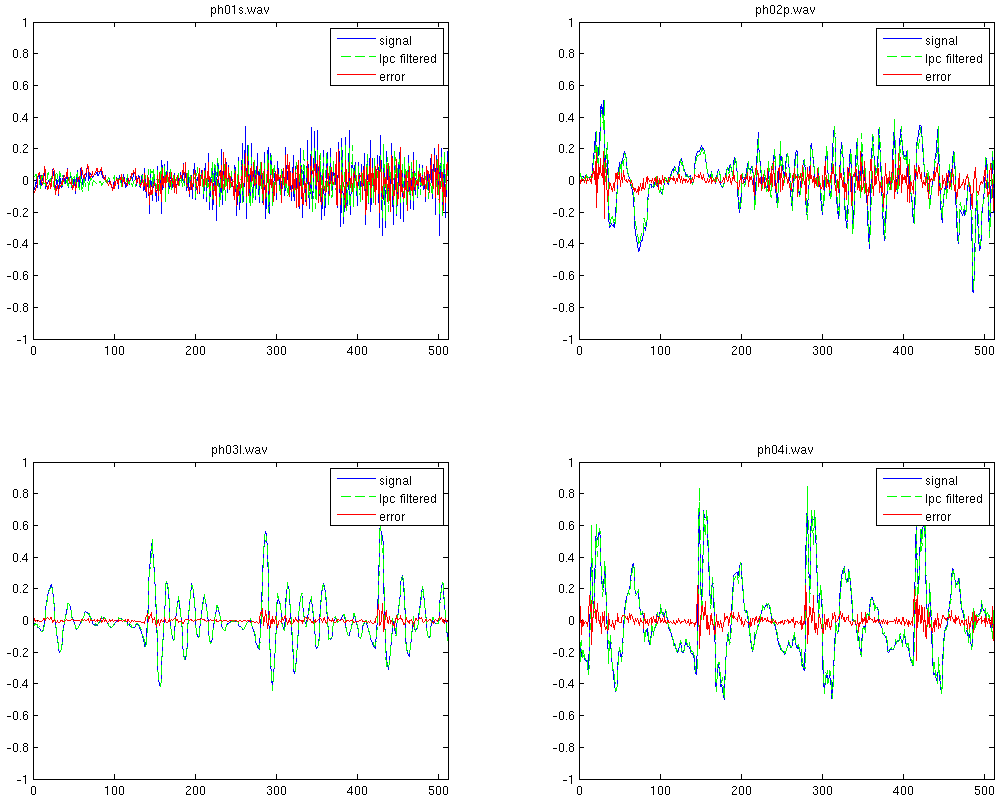
\includegraphics[scale=0.45]{sig_lpc_err2.png}

\subsubsection*{(1)}

The function \TT{plot\_lpc} can be used to plot a single graphic given the
signal, the filtered signal and the error. The function \TT{plot\_all} reads
all wav files, truncates them to 512 samples and calls \TT{plot\_lpc}.

\subsubsection*{(2)}

\begin{itemize}
  \item The \TT{s} signal is mostly hissing noise, so it can not be very well
  predicted. That is why the error is so big; \\
  \item The \TT{p} signal is better in this respect, but compared to \TT{l} and
  \TT{i} has sharper spikes, and big error; \\
  \item The \TT{l} signal is smooter, and the error is high just when it has
  a taller spike; \\
  \item The \TT{i} is a little bit worse than \TT{l} -- it has a lot of small
  local spikes and a few big ones. The error is small except for the big
  spikes. \\
\end{itemize}

\subsection*{1.4}

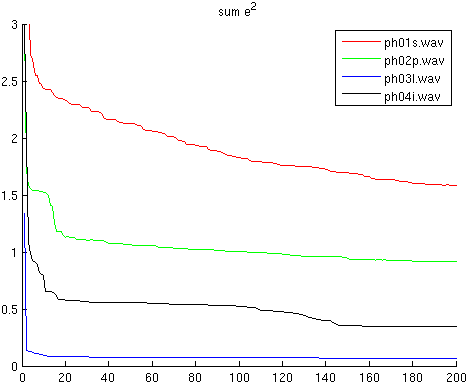
\includegraphics[scale=1]{error2.png}

\subsubsection*{(1)}

The script \TT{plot\_error} calculates the errors for all given P's and signals
and plots them together on a single plot.

\subsubsection*{(2)}

All errors stabilize for $ P \le 20 $, except \TT{s}, because it is almost
random, so the more coefficients are added the better the approximation.

\end{document}
